\subsection{Data Visualisation}
	It is helpful to visualise our data to confirm the presence of any detectable patterns and/or to help improve our learning algorithms. Since our Principal Component Analysis revealed that we need at least 100 principal components to capture at least half of the variance, it is not illustrative to visualise our data by plotting the data points on a 2D plane using only the first two principal components. Instead, we take the six corresponding bins of spectrograms of the two classes of annotations (apnoea, no apnoea) and take the average for each class as shown in Figure \ref{fig:spectrogramClassesVisualise}. We can notice the differences in the spectrograms which is reassuring because we can see that there exist some patterns to be found and that the spectrogram contains enough information to detect sleep apnoea.
	\begin{figure}[ht!]
		\centering
			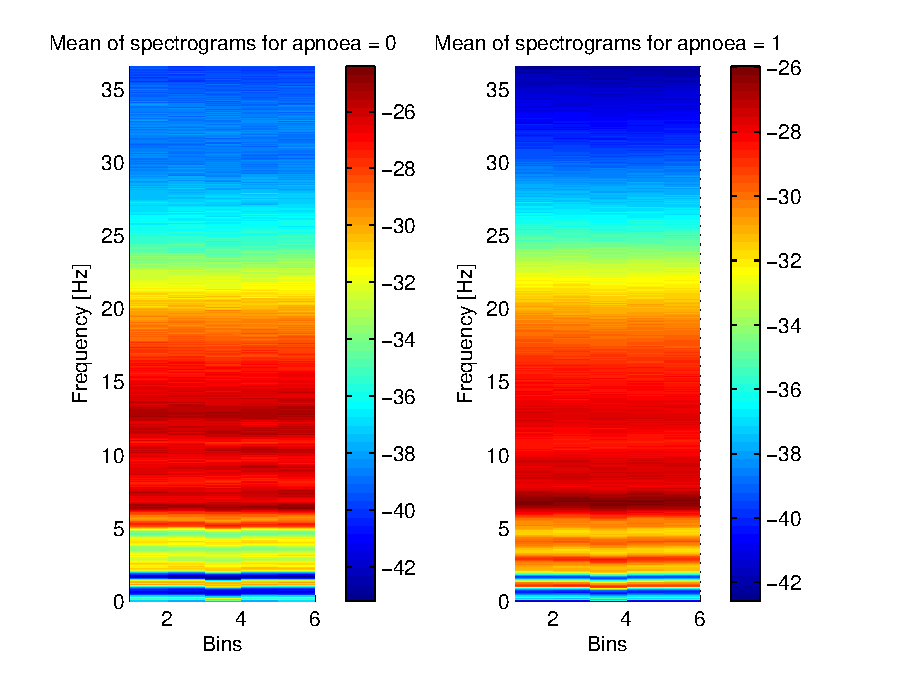
\includegraphics{drawings/spectrogramClassesVisualise.eps}
		\caption{Comparison of the spectrograms of the two classes based on their average spectrogram from the first five records.}
		\label{fig:spectrogramClassesVisualise}
	\end{figure}